% !TEX encoding = UTF-8 Unicode
% !TEX TS-program = XeLaTeX
\documentclass[utf8,10pt]{beamer}

% ------------------------------- Couleurs ----------------------------------------
% http://latexcolor.com
% https://kuler.adobe.com/fr
\definecolor{cadmiumgreen}{rgb}{0.0, 0.42, 0.24}
\definecolor{StanfordRed}{rgb}{0.65625, 0.0, 0.0078125}
\definecolor{StandfordBlue}{RGB}{12, 76, 116}
\definecolor{StandfordGreen}{RGB}{0, 90, 25}

% ------------------------------- Apparence de Beamer ---------------------------
% \usepackage{beamerthemesplit} // Activate for custom appearance
%\usetheme{Hannover}
%\usecolortheme{beaver}
%\useinnertheme{nom du theme interne}
%\useoutertheme{nom du theme externe}

\setbeamercolor{structure}{fg=StanfordRed, bg=white}
%\setbeamercolor{normal text}{fg=black,bg=white}
\setbeamercolor{alerted text}{fg=StandfordGreen}
\setbeamercolor{example text}{fg=StanfordRed}
%\setbeamercolor{background canvas}{parent=normal text}

% -------------------------- Paramétrage de Beamer ---------------------------
\setbeamertemplate{frametitlecontinuation}{\insertcontinuationcountroman} % Texte sur plusieurs frames
\setbeamerfont{page number in head/foot}{size=\normalsize}
\setbeamertemplate{footline}[frame number]{}
\setbeamertemplate{navigation symbols}{}

% ------------------------------- Paramétrage du pdf -------------------------------
\hypersetup{pdfpagemode=FullScreen}

% --------------------------- Création de boutons liens ----------------------------
% \hyperlink{cible}{aller à la cible}
% \hyperlink{cible}{\beamerbutton{y aller aussi}}
% boutons utilisables :
% \beamergotobutton    \beamerreturnbutton    \beamerskipbutton

% -------------------------------- Polices, langue et entrée au clavier -------------
\usepackage[french]{babel}

\usefonttheme{professionalfonts} % using non standard fonts for beamer
\usefonttheme{serif} % default family is serif
\usepackage{fontspec}
%\setmainfont{Utopia}


% -------------- Hyphenation plus proche de celle de LaTeX ------------------------
%\usepackage{ragged2e}
%\let\raggedright=\RaggedRight

% -------------------------- Listes énumérées ------------------------------------
\setbeamertemplate{enumerate item}[default] % Valeurs possibles : default, circle, square ou ball
%\setbeamertemplate{enumerate subitem}[square]
%\setbeamertemplate{enumerate subsubitem}[square]

% Possibilité de paramétrer chaque liste individuellement
%\begin{enumerate}[option] % i, a, a.) ...
%
%\end{enumerate}

% ------------------------------- Listes ---------------------------------------
\setbeamertemplate{itemize item}[default]
%\setbeamertemplate{itemize subitem}[style]
%\setbeamertemplate{itemize subsubitem}[style]
%style = default, triangle, circle, square et ball

% -------------------------------- Blocs ---------------------------------------
\setbeamertemplate{blocks}[rounded][shadow=true] % peut être inséré dans le document
%\begin{block}{Bloc arrondi}
%  Un bloc avec option rounded, avec shadow.
%\end{block}

%\begin{alertblock}{Un bloc très alerte}
%  Texte du block \texttt{alertblock}
%\end{alertblock}
%
%\begin{exampleblock}{Un bloc exemplaire}
%    Exemple de block \texttt{exampleblock}
%\end{exampleblock}


% -------------------------------- Boîtes ---------------------------------------
%\beamerboxesdeclarecolorscheme{clair}{couleur1}{couleur2}
%\beamerboxesdeclarecolorscheme{autre}{couleur3}{couleur4}
%\begin{beamerboxesrounded}[scheme=clair,shadow=true]{Un bloc arrondi}
%     texte
%\end{beamerboxesrounded}
\beamerboxesdeclarecolorscheme{clair}{StandfordBlue}{StandfordBlue!10}
\beamerboxesdeclarecolorscheme{autre}{StandfordGreen}{StandfordGreen!10}

% ------------------------------ Deux colonnes -----------------------------------
%\begin{columns}[T]
%    \begin{column}{5cm}
%        \begin{example} % boite mais cela pourrait-être du texte
%            Let's dance!
%        \end{example}
%    \end{column}
%    
%    \begin{column}{5cm}
%        \begin{alertblock}{Super important !} % idem
%            Let's dance!
%        \end{alertblock}
%    \end{column}
%\end{columns}

% ----------------------- Découverte progressive d'une liste ----------------------
%\begin{itemize}[<+->]
%
%\end{itemize}

% ----------------------- Coloration du code ------------------------------------
\usepackage{verbments}
\plset{language=python,%
        style=tango,%
        listingname=\textbf{Code},%
        listingnamefont=\sffamily\bfseries\color{white},%
        captionfont=\sffamily\color{white},%
        captionbgcolor=StandfordBlue,%
        numbers=left,%
        numbersep=5pt,%
        fontsize=\small,%
        fvset={frame=leftline,framerule=3pt,rulecolor=\color{StandfordBlue}},%
        mathescape=true,%
        texcl=true}

% ------------------------ Graphiques -----------------------------------------
\usepackage{graphicx}

% ________________________ Tables ------------------------------------------
\usepackage{booktabs} % permet l'utilisation de toprule, midrule, bottomrule

% ------------------------- Informations sur la présentation -------------------
\title{Éléments d'histoire et d'architecture des ordinateurs}
\subtitle{Chapitre 01}
\author{1 NSI}
\date{}

% ------------------------- Macros ------------------------------------------------
\newcommand{\el}[1]{\hfill #1 \hfill}

% ------------------------------- Début du document ---------------------------------
\begin{document}

% --------------------------------- Page de titre -----------------------------------
\begin{frame}
    \titlepage
\end{frame}


% ------------------------- Sommaire principal --------------------------------------
\section*{Plan}
\begin{frame}

	\frametitle{Plan}
	
	\tableofcontents
\end{frame}

% ------------------------- Section --------------------------------------
\section{Langages et ordinateurs}

% ------------------------- Sommaire première section --------------------------------------
\begin{frame}

	\frametitle{Plan}
	
	\tableofcontents[currentsection]
\end{frame}

% ------------------------- Sous-section --------------------------------------
\subsection{Vocabulaire}
% ------------------------- Diapo ---------------------------------------
\begin{frame}
    \frametitle{Vocabulaire}
    \begin{itemize}
        \item Un \alert{ordinateur} est une machine capable d'exécuter des actions
        à partir d'instructions préalablement définies.
        
        \item La suite des instructions décrivant la façon dont l'ordinateur doit effectuer
        un certain travail est appelé \alert{programme}.
        
        \item Un \alert{algorithme} est une suite finie et non ambigüe d'opérations ou 
        d'instructions permettant de résoudre un problème.
        
        \item Un programme est généralement constitué de plusieurs algorithmes exprimés dans un
        \alert{langage de programmation}.
    \end{itemize}
    
    \begin{exampleblock}{Remarque}
        Différents programmes peuvent implémenter des algorithmes différents pour résoudre
        le même problème.
    \end{exampleblock}
\end{frame}

% ------------ Diapo ------------------
\begin{frame}
	\frametitle{Pourquoi ne pas utiliser un langage humain ?}
	
	Les langages humains sont :
	\begin{itemize}
		\item \textbf{Complexes :} il nous faut de longues années d'étude avant d'être capables de maitriser notre langue maternelle
		\item \textbf{Ambigüs :} de nombreux mots changent de sens en fonction du contexte dans lequel ils sont utilisés
		\item \textbf{Évolutifs :} les langages évoluent au cours du temps avec les sociétés qui les utilisent 
	\end{itemize}
	
	\begin{exampleblock}{Exemple}
	Example is taken from the instructions with a shipment of ballistic missiles from the British Admiralty:
	
		\emph{"It is necessary for technical reasons that these warheads be stored upside down, that is, with the top at the bottom and the bottom at the top. In order that there be no doubt as to which is the bottom and which is the top, for storage purposes, it will be seen that the bottom of each warhead has been labeled ’TOP’."}
	\end{exampleblock}
\end{frame}

% ------------------------- Sous-section --------------------------------------
\subsection{Langage machine}

% ------------------------- Sommaire deuxième section --------------------------------------
\begin{frame}

	\frametitle{Plan}
	
	\tableofcontents[currentsubsection]
\end{frame}

% ------------------------- Diapo ---------------------------------------
\begin{frame}[allowframebreaks=0.95]
    \frametitle{Langage machine}
    \begin{itemize}
        \item Les circuits électroniques de chaque ordinateur ne peuvent reconnaître et exécuter
    directement qu'un nombre très limité d'instructions.
        \begin{description}
            \item[Exemple :]
            \begin{itemize}
                \item Additionner deux nombres ;
                \item Vérifier si un nombre est égal à zéro ;
                \item Changer d'emplacement une donnée, dans la mémoire.
            \end{itemize}
        \end{description}

        \item L'ensemble des instructions exécutables \alert{directement} par un ordinateur forme
        un langage appelé \alert{langage machine}.
        \hyperlink{http://fr.wikipedia.org/wiki/Langage_machine}{\beamergotobutton{Wikipedia}}
    \end{itemize}
    
    \begin{exampleblock}{Remarque}
        Lorsqu'on conçoit un nouvel ordinateur, il est nécessaire de choisir l'ensemble des instructions
        qui formeront son langage machine.  En général, on cherche à ce que ces instructions soient les
        plus simples possibles, compte tenu des performances attendues de la machine, \alert{afin de réduire
        la complexité}, et donc le coût, des circuits électroniques nécessaires.
    \end{exampleblock}
    
    \begin{itemize}
        \item Caractéristiques du \alert{langage machine} qui le rendent pénible et fastidieux à utiliser :
        \begin{itemize}
            \item Il est \alert{numérique}. La séquence 249 75 42 pourrait par exemple signifier \og
            Stocker le caractère K à l'adresse 42, dans la mémoire\fg\ ;
            
            \item Les opérations de base sont tellement limitées qu'il faut en combiner un très grand nombre
            pour résoudre le moindre problème ;
            
            \item Deux modèles différents d'ordinateurs n'ont pas le même langage machine.
            
        \end{itemize} 
    \end{itemize}
    
    Pour résoudre ce problème, on définit un nouveau jeu d'instructions, plus pratique à utiliser pour le 
    programmeur. 
    
    On obtient ainsi de nouveaux langages dits de \og haut niveau. \fg\footnote{La vision de 
    l'architecture d'un ordinateur présentée ici est extrêmement simpliste.}\footnote{\og de plus haut niveau \fg{}
    fait référence au modèle en couches de l'architecture d'un ordinateur : plus on s'élève, plus on s'éloigne
    du langage machine.}\\[6pt]
    \hfill \hyperlink{http://fr.wikipedia.org/wiki/Langage_de_haut_niveau}{\beamergotobutton{Wikipedia}}
\end{frame}

% ------------------------- Diapo ---------------------------------------
\begin{frame}
    \frametitle{Langage machine --- exemple}
    
    Instructions en langage machine (les 0 et les 1 ont été remplacés par une écriture hexadécimale, 4 fois plus condensée) indiquant à l’ordinateur d’écrire \og Hello World! \fg{} à l’écran.    
    \begin{block}{}
...\\
48 83 ec 08 e8 73 00 00  00 e8 02 01 00 00 e8 ed \\
01 00 00 48 83 c4 08 c3  ff 35 ba 04 20 00 ff 25 \\
bc 04 20 00 0f 1f 40 00  ff 25 ba 04 20 00 68 00 \\
00 00 00 e9 e0 ff ff ff  ff 25 b2 04 20 00 68 01 \\
31 ed 49 89 d1 5e 48 89  e2 48 83 e4 f0 50 54 49 \\
c7 c0 80 05 40 00 48 c7  c1 f0 04 40 00 48 c7 c7 \\
eb b0 06 60 00 48 c1 fb  03 48 83 eb 01 48 39 d8 \\
73 24 66 0f 1f 44 00 00  48 83 c0 01 48 89 05 25 \\
48 89 6c 24 d8 4c 89 64  24 e0 48 8d 2d 9b 01 20 \\
00 4c 8d 25 94 01 20 00  4c 89 6c 24 e8 4c 89 74 \\
24 f0 4c 89 7c 24 f8 48  89 5c 24 d0 48 83 ec 38 \\
4c 29 e5 41 89 fd 49 89  f6 48 c1 fd 03 49 89 d7 \\
...
    \end{block}

    \end{frame}

% ------------------------- Diapo ---------------------------------------
\begin{frame}[fragile]
    \frametitle{Langages d'assemblage --- exemple}

\begin{columns}[t]
    \begin{column}{0.49\textwidth}
            \begin{block}{}
\begin{pyglist}[language=shell] 
    .file   "test.c"
    .section        .rodata
.LC0:
    .string "Hello World!\n"
    .text
.globl main
    .type   main, @function
main:
.LFB0:
    .cfi_startproc
    pushq   %rbp
    .cfi_def_cfa_offset 16
    .cfi_offset 6, -16
    movq    %rsp, %rbp 
\end{pyglist}       
        \end{block}
    \end{column}
    
    \hfill
    
    \begin{column}{0.49\textwidth}
        \begin{block}{} 
\begin{pyglist}[language=shell] 
    .cfi_def_cfa_register 6
    movl    $13, %edx
    movl    $.LC0, %esi
    movl    $1, %edi
    call    write
    movl    $0, %eax
    leave
    .cfi_def_cfa 7, 8
    ret
    .cfi_endproc
.LFE0:
    .size    main, .-main
    .ident   "GCC: (GNU)"
    .section  .note.GNU-stack,
                  "",@progbits
\end{pyglist}
        \end{block}
    \end{column}
\end{columns}

\end{frame}

% ------------------------- Diapo ---------------------------------------
\begin{frame}[fragile]
    \frametitle{Langages de haut niveau --- exemples en C et python}
    \begin{columns}[t]
    
    \begin{column}{0.49\textwidth}
        \begin{block}{En C}
            \begin{pyglist}[language=C]
#include<stdio.h>
            
int main() {
printf("hello, world");
return 0;
}
            \end{pyglist}
        \end{block}

    \end{column}
    
    \hfill
    
    \begin{column}{0.49\textwidth}
        \begin{block}{En python}
            \begin{pyglist}[language=python]
#!/bin/env python
# -*- coding: utf8 -*-
            
print("hello, world")

            \end{pyglist}
        \end{block}
    \end{column}
    \end{columns}
    
    \begin{alertblock}{Remarque}
    Les langages de \og haut niveau \fg{} ne sont pas numériques mais se rapprochent
    des langues parlées par les humains.
    \end{alertblock}

\end{frame}


% ------------------------- Sous-section --------------------------------------
\subsection{Traduction, interprétation}

% ------------------------- Sommaire deuxième section --------------------------------------
\begin{frame}

	\frametitle{Plan}
	
	\tableofcontents[currentsubsection]
\end{frame}

% ------------------------- Diapo ---------------------------------------
\begin{frame}
    \frametitle{Traduction, interprétation}
    
    \begin{exampleblock}{À garder à l'esprit}
        Un ordinateur ne peut exécuter que des instructions écrites dans son langage machine.
    \end{exampleblock}
    
    \vfill
    
    Lorsqu'un programme est écrit dans un langage de \og haut niveau \fg , il est nécessaire
    de le transformer en langage machine. Deux techniques existent :
    \begin{itemize}
        \item la \alert{traduction}.\\ Le programme qui traduit un langage de \og haut niveau \fg{}
        s'appelle un \alert{compilateur}.
        \item l'\alert{interprétation}\\ Le programme qui interprète un langage s'appelle \ldots 
        un \alert{interpréteur}.
    \end{itemize}

\end{frame}

% ------------------------- Diapo ---------------------------------------
\begin{frame}
    \frametitle{Traduction I}
    \begin{block}{}
    \begin{center}
        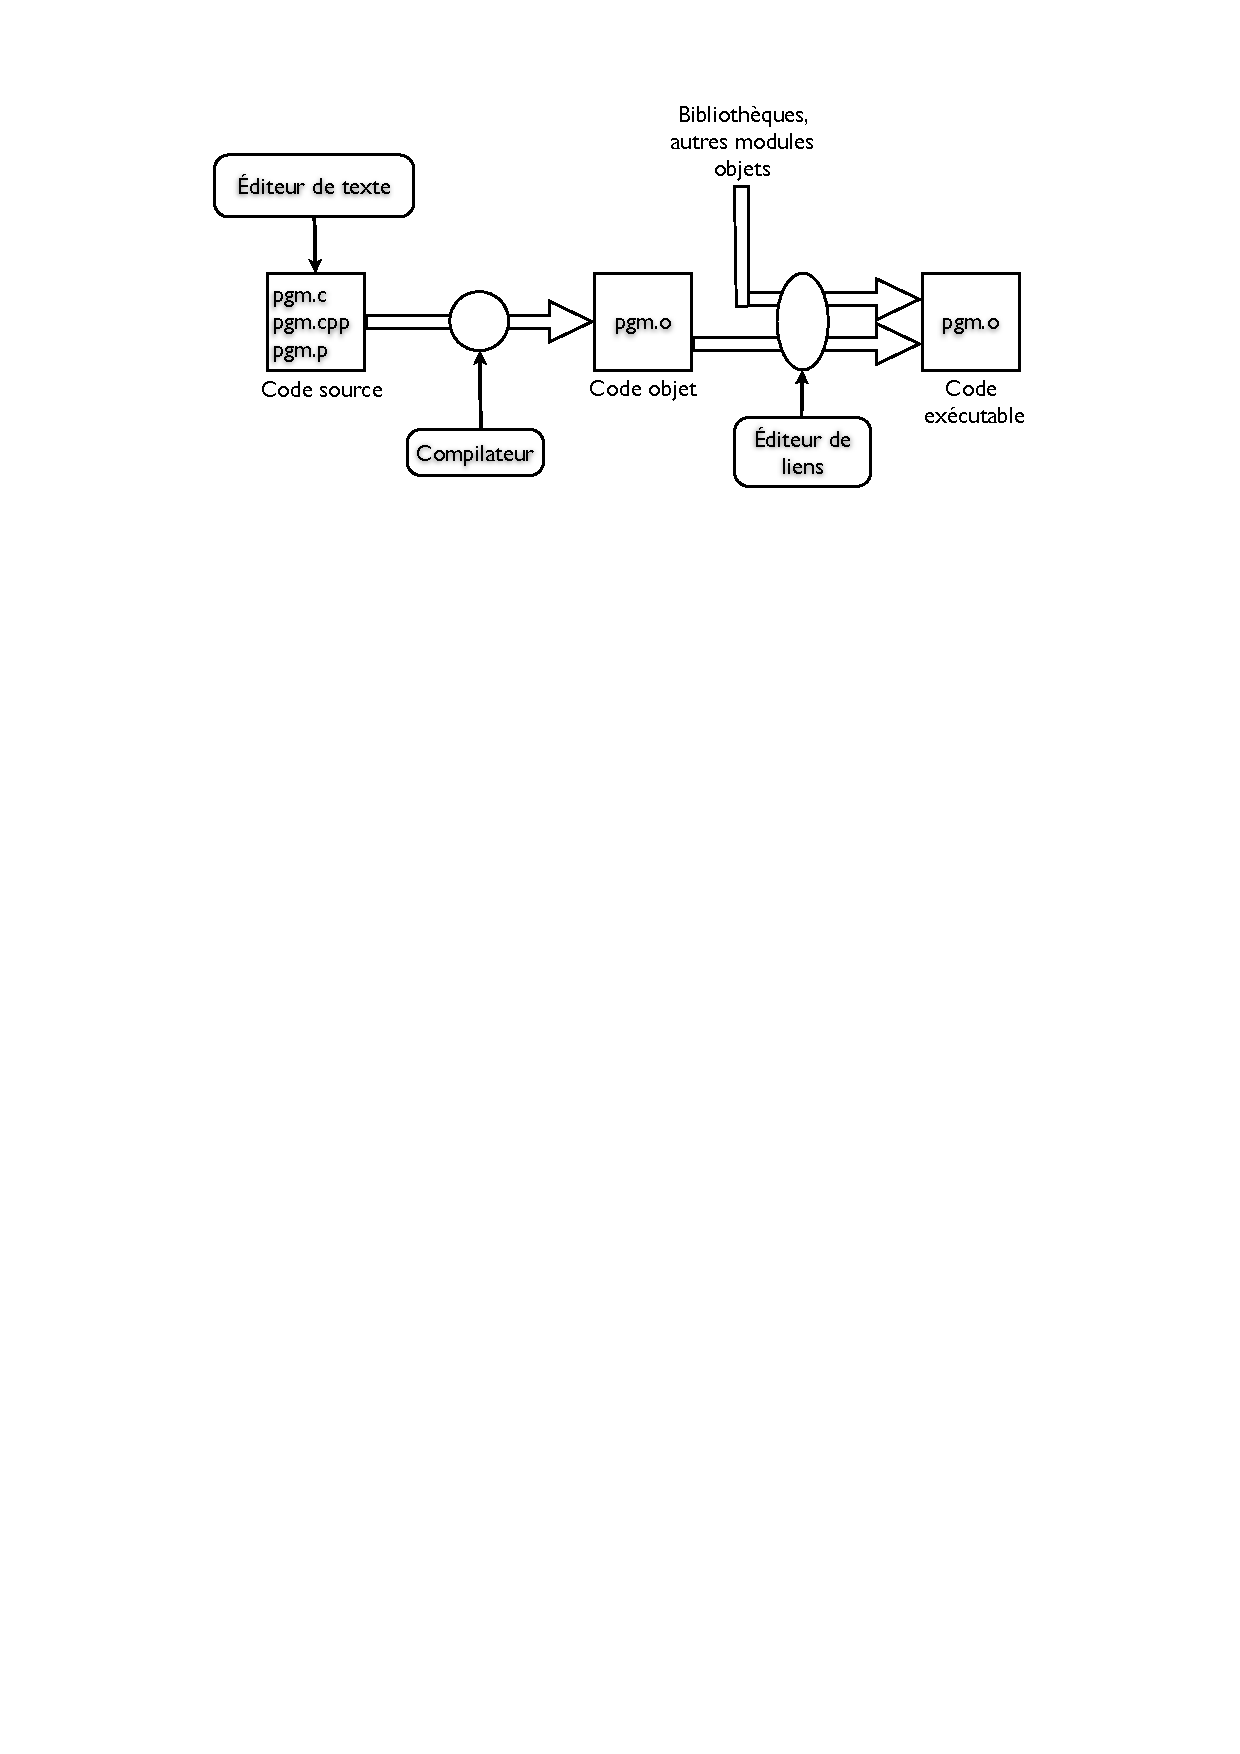
\includegraphics[scale=0.5]{./images/Compilation}
    \end{center}
    \end{block}
    
    \begin{enumerate}
        \item Un compilateur (associé à un éditeur de liens) transforme le code source écrit en langage 
        évolué en un fichier contenant du code exécutable formé de codes numériques propres à la machine. 
        \alert{Le code source
         est analysé dans son ensemble avant cette traduction}.
         \item Le programme peut-être lancé à tout moment, une fois la compilation réalisée.
    \end{enumerate}
\end{frame}

% ------------------------- Diapo ---------------------------------------
\begin{frame}
    \frametitle{Traduction II}
    \begin{description}
        \item[Avantages :]\hspace{1cm}\\
        \begin{itemize}
            \item Le code engendré est directement exécuté par la machine physique.
            \item Le compilateur peut optimiser le code lors de la phase de compilation.
            \item Le compilateur peut effectuer un certain nombre de vérifications lors de la phase de 
            compilation (en particulier la cohérence des \alert{types}).
            \item Le programme est plus « portable » que dans le cas du langage machine : en cas 
            d’utilisation d’une nouvelle architecture, il « suffit » de compiler à nouveau le code source.
        \end{itemize}
    \end{description}

\end{frame}

% ------------------------- Diapo ---------------------------------------
\begin{frame}
    \frametitle{Traduction III}
    \begin{description}
        \item[Inconvénients :]\hspace{1cm}\\
        \begin{itemize}
            \item Il n’est pas toujours facile de relier une erreur d’exécution au code source.
            \item Toute modification du code source impose de compiler à nouveau le programme (processus 
            qui peut s'avérer être très long).
            \item Toute utilisation sur une nouvelle architecture (structure de l'ordinateur et système
            d'exploitation) impose de compiler à nouveau le programme.
        \end{itemize}
    \end{description}

\end{frame}

% ------------------------- Diapo ---------------------------------------
\begin{frame}
    \frametitle{Interprétation I}
    \begin{block}{}
    \begin{center}
        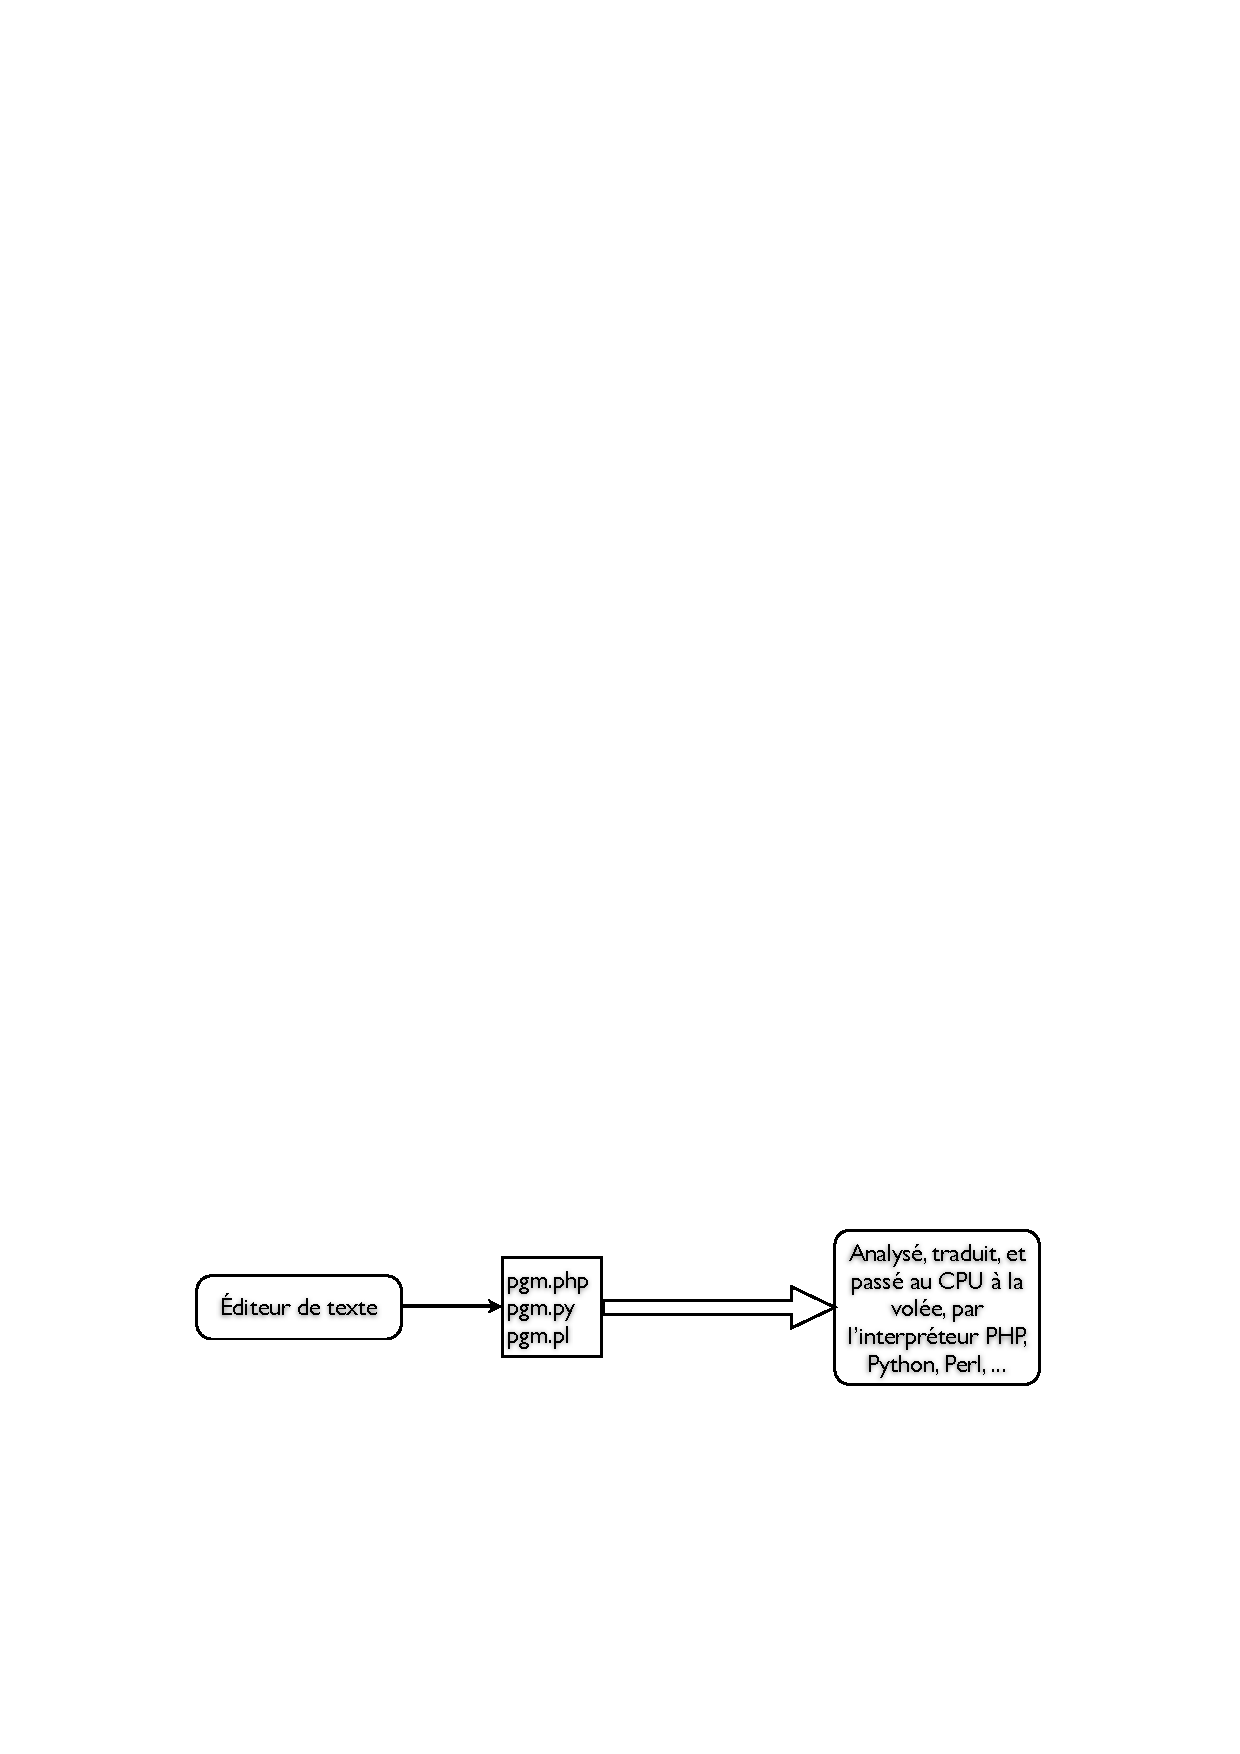
\includegraphics[scale=0.5]{./images/Interprétation}
    \end{center}
    \end{block}
    
    Un interpréteur \alert{analyse} le code source d’un programme, le \alert{traduit} en langage machine
     et fait exécuter le code par l’ordinateur.\\
    La grande différence avec un compilateur est qu’il effectue ces tâches  \alert{au fur et à mesure} :
    \begin{enumerate}
        \item Il lit une instruction et l’analyse.
        \item Il traduit l’instruction en langage machine (si l'analyse n'a révélé aucune erreur).
        \item Il fait exécuter le code machine.
    \end{enumerate}
    
\end{frame}

% ------------------------- Diapo ---------------------------------------
\begin{frame}
    \frametitle{Interprétation II}
    \begin{description}
        \item[Avantages :]\hspace{1cm}\\
        \begin{itemize}
            \item Le programme peut fonctionner sans modification du code source sur plusieurs architectures. 
            \item Le développement d’un logiciel prend généralement beaucoup moins de temps (on évite la 
            phase de compilation).
            \item Le lien entre instruction et exécution étant plus direct, il peut être plus facile 
            de relier une erreur d’exécution au texte source.
            \item Il est généralement plus facile \og d’étudier \fg{} le fonctionnement du programme.
        \end{itemize}
    \end{description}
    
\end{frame}


% ------------------------- Diapo ---------------------------------------
\begin{frame}
    \frametitle{Interprétation III}
    \begin{description}
        \item[Inconvénients :]\hspace{1cm}\\
        \begin{itemize}
            \item L’interpréteur simulant le fonctionnement de l’ordinateur, les programmes sont 
            généralement beaucoup moins rapides (x10 à x100) que les programmes compilés.
            \item Il est nécessaire d’installer l’interpréteur adapté à la plateforme pour pouvoir 
            exécuter le programme (sous réserve qu'il existe).
        \end{itemize}
    \end{description}
    
\end{frame}


% ------------------------- Diapo ---------------------------------------
\begin{frame}
    \frametitle{Exécution mixte}
    \begin{block}{}
    \begin{center}
        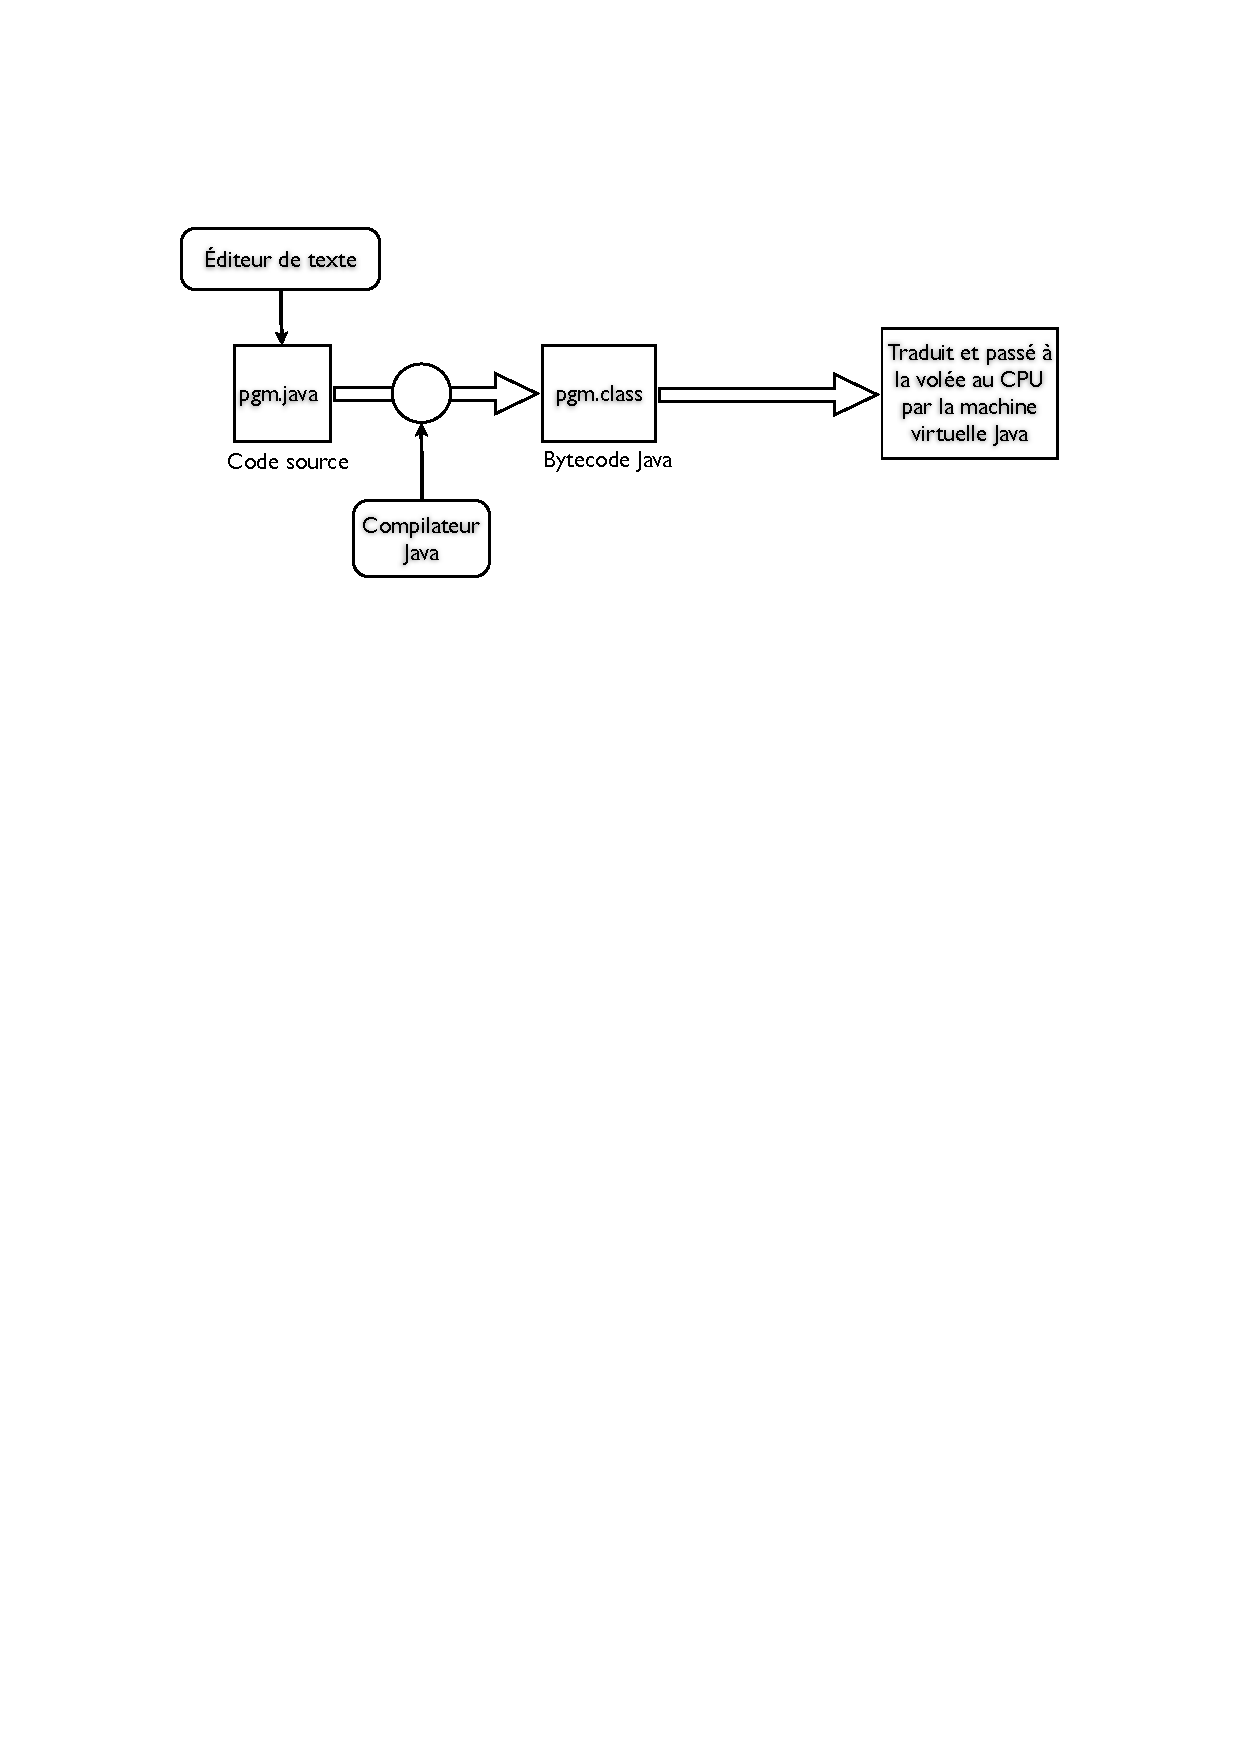
\includegraphics[scale=0.4]{./images/Execution-mixte}
    \end{center}
    \end{block}
    
    La programmation en Java utilise les deux techniques précédentes :
    \begin{enumerate}
        \item Un fichier source en Java est tout d’abord compilé, mais le compilateur, au lieu de générer 
        des instructions directement exécutables par le processeur utilisé, produit un code (\alert{Bytecode})
         spécifique à une \alert{machine virtuelle}\footnote{C'est le langage machine de cette machine virtuelle.}
         \item Un interpréteur (jre pour Java Runtime Environment), spécifique à chaque architecture, interprète par la suite ce code en langage machine\footnote{Le Bytecode est proche du langage d'assemblage, cette interprétation est relativement rapide.}.

    \end{enumerate}
\end{frame}

% ------------------------- Subsection ----------------------------------------------
\subsection{Matériel et logiciel}

% ------------------------- Sommaire deuxième section --------------------------------------
\begin{frame}

	\frametitle{Plan}
	
	\tableofcontents[currentsubsection]
\end{frame}

% --------------------------- Diapo --------------------------------------------------
\begin{frame}
    \frametitle{Matériel et logiciel}
    
    \begin{exampleblock}{À méditer\ldots}
    \begin{itemize}
        \item Matériel et logiciel sont logiquement équivalents.
        
        \item Ce qui est matériel aujourd'hui pourra être logiciel demain, et réciproquement.
        
        \item Ce qui est matériel chez l'un peut être logiciel chez l'autre.
    \end{itemize}
     
    \end{exampleblock}
    
    

\end{frame}


% ------------------------- Section --------------------------------------
\section{Quelques étapes de l'évolution de l'architecture des ordinateurs}

% ------------------------- Sommaire deuxième section --------------------------------------
\begin{frame}

	\frametitle{Plan}
	
	\tableofcontents[currentsection]
\end{frame}

% ------------------------- Subsection ----------------------------------------------
\subsection{Les calculateurs mécaniques (1642 -- 1945)}

% ------------------------- Diapo ----------------------------------------------
\begin{frame}
    \frametitle{Blaise Pascal (1646 -- 1716)}
    \begin{center}
        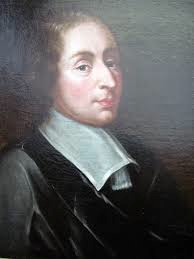
\includegraphics[scale=0.4]{./images/pascal.png}
        \hfill
        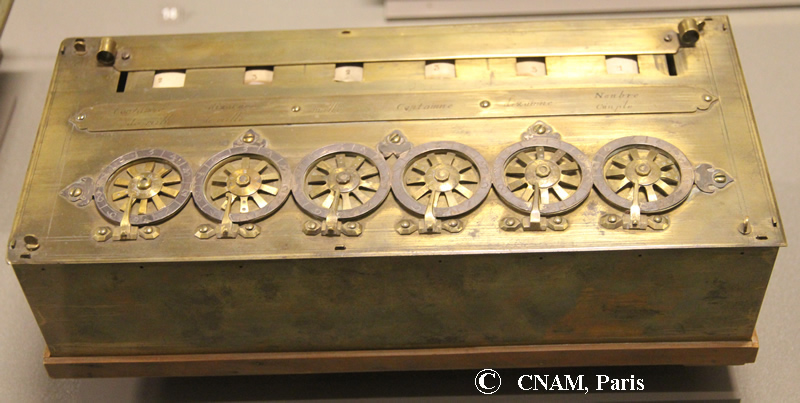
\includegraphics[scale=0.25]{./images/pascaline.jpg}
    \end{center}
    
    \begin{itemize}
        \item Agé de 19 ans, Pascal\footnote{C'est en son honneur que Niklaus Wirth a appelé Pascal un des 
    langages de programmation qu'il a inventé.} a construit une machine entièrement mécanique, à 
    base d'engrenages et actionnée à la main, destinée à aider son père, intendant des finances
    en haute Normandie.
        \item Cette machine effectuait les additions et les soustractions.
    \end{itemize}
    
    \hfill \hyperlink{http://fr.wikipedia.org/wiki/Blaise_Pascal}{\beamergotobutton{Wikipedia}}
\end{frame}

% ------------------------- Diapo ----------------------------------------------
\begin{frame}
    \frametitle{Gottfried Wilhelm Leibniz (1623 -- 1662)}
    \begin{center}
        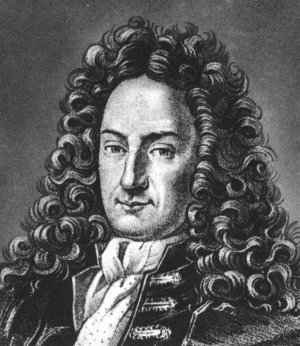
\includegraphics[scale=0.38]{./images/Leibniz.jpg}
        \hfill
        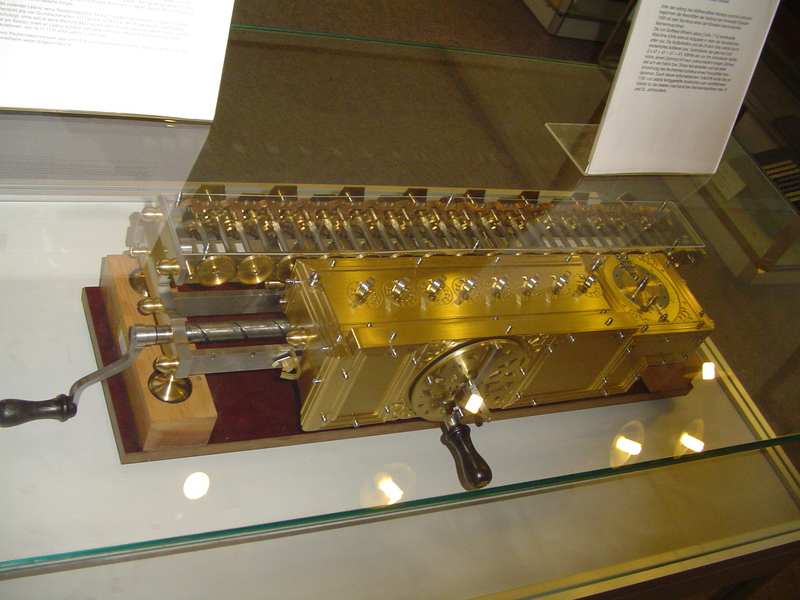
\includegraphics[scale=0.22]{./images/machine-leibniz.jpg}
    \end{center}
    
    \begin{itemize}
         
        \item Leibniz a ajouté la multiplication et la division à la machine de Pascal.
    \end{itemize}
    
    \hfill \hyperlink{http://fr.wikipedia.org/wiki/Gottfried_Wilhelm_Leibniz}{\beamergotobutton{Wikipedia}}
\end{frame}

% ------------------------- Diapo ----------------------------------------------
\begin{frame}
    \frametitle{Charles Babbage (1792 -- 1871) I}
    \begin{center}
        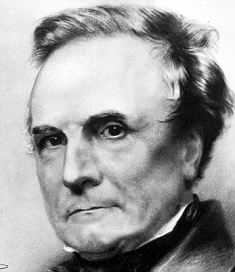
\includegraphics[scale=0.22]{./images/Babbage}
        \hfill
        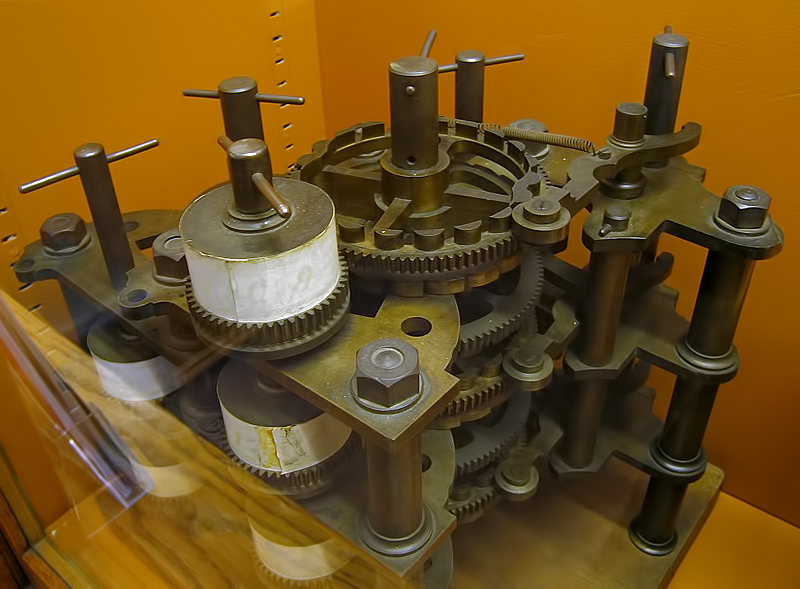
\includegraphics[scale=0.22]{./images/BabbageDifferenceEngine}
    \end{center}
    
    \hfill \hyperlink{http://fr.wikipedia.org/wiki/Babbage}{\beamergotobutton{Wikipedia}}
\end{frame}

% ------------------------- Diapo ----------------------------------------------
\begin{frame}
    \frametitle{Charles Babbage (1792 -- 1871) II}
        
        \begin{center}
        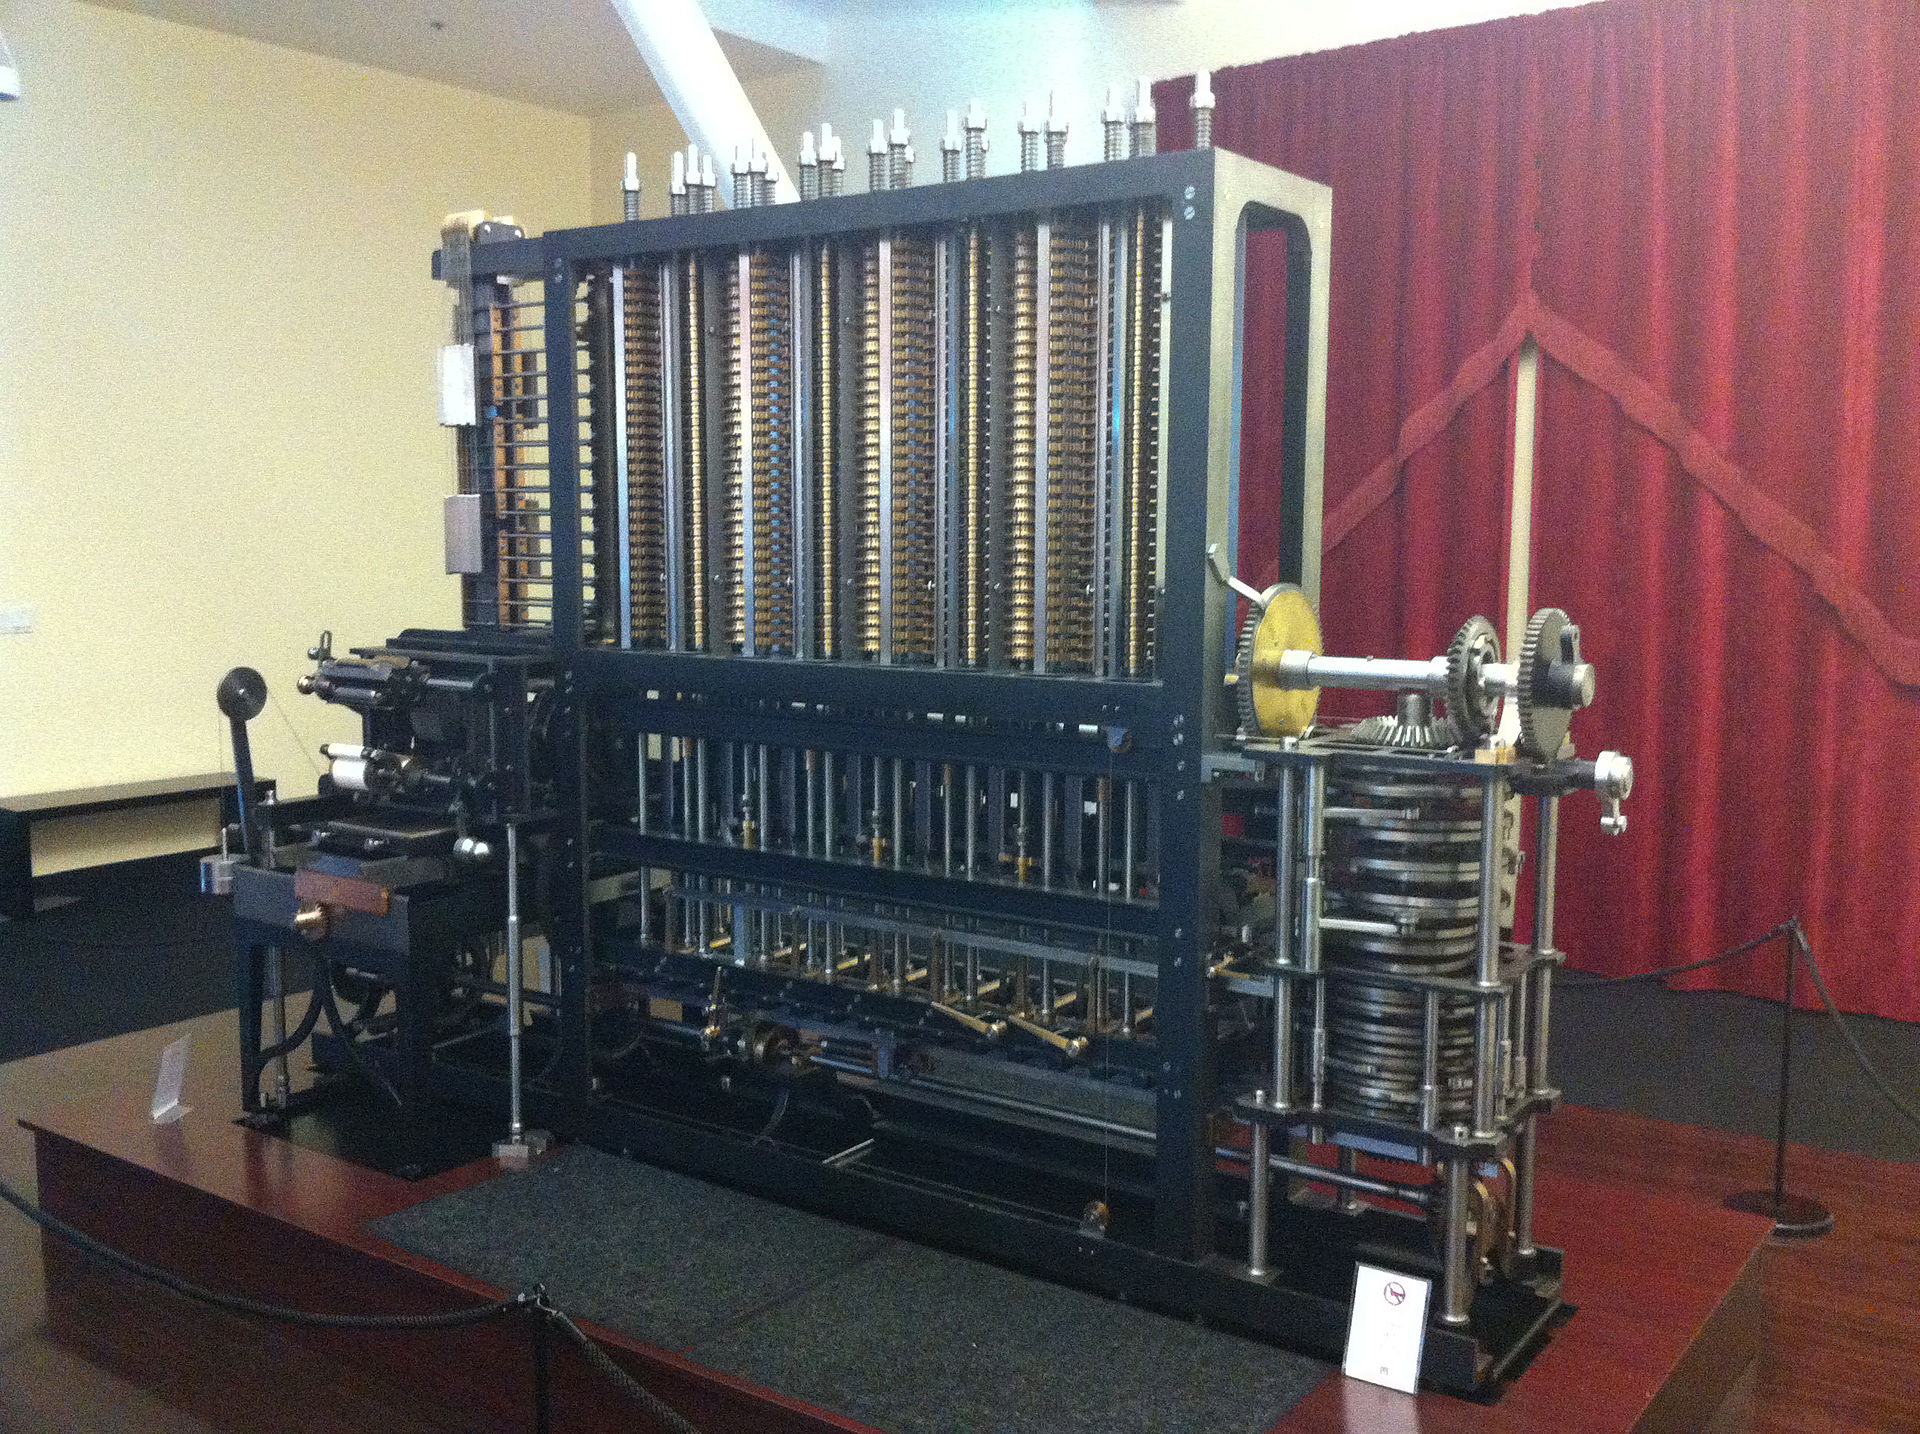
\includegraphics[scale=0.35]{./images/machine-babbage}
        \hfill
        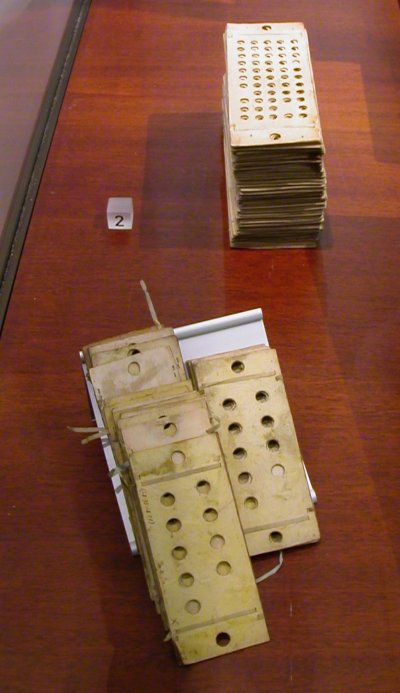
\includegraphics[scale=0.9]{./images/PunchedCardsAnalyticalEngine}
    \end{center}
    
\end{frame}

% ------------------------- Diapo ----------------------------------------------
\begin{frame}
    \frametitle{Charles Babbage (1792 -- 1871) III}
    \framesubtitle{Machine à différences}
    
    \begin{itemize}
        \item Cette machine effectuait les additions et 
        les soustractions et était destinée à établir des tables numériques pour la 
        navigation en mer. 
        
        \item Cette machine n'exécutait qu'un seul programme consistant à 
        \og calculer les polynômes en utilisant le calcul différentiel !\fg.
        
        \item \alert{Originalité} : pour retourner les résultats de ses calculs la machine gravait 
        un plateau de cuivre à
        l'aide d'un timbre en acier, préfigurant ainsi les médias non réinscriptibles comme les 
        cartes perforées ou les premiers disques optiques. 
    \end{itemize}

\end{frame}

% ------------------------- Diapo ----------------------------------------------
\begin{frame}
    \frametitle{Charles Babbage (1792 -- 1871) IV}
    \framesubtitle{Machine analytique}
    
    \begin{itemize}
        \item Cette machine comportait quatre parties :
        \begin{itemize}
            \item le magasin (la mémoire)
            \item le moulin (l'unité de calcul)
            \item l'entrée (le lecteur de cartes perforées\footnote{Babbage a eu l'idée d'utiliser 
            des cartes du \alert{métier Jacquard} \hyperlink{http://fr.wikipedia.org/wiki/Métier_Jacquard}%
            {\beamergotobutton{Wikipedia}}.})
            \item la sortie (perforation ou impression)
        \end{itemize}
        
        \item Le magasin disposait de 1\,000 mots de 50 chiffres décimaux que l'on pouvait utiliser
        pour stocker variables et résultats.
        
        \item Le moulin prenait les opérandes provenant du magasin, en faisait l'addition, la soustraction,
        la multiplication ou la division et renvoyait le résultat vers le magasin\footnote{Rappel : tout 
        était mécanique !}.
        
        \item Certaines instructions pouvaient commander de faire le test d'un nombre et provoquer
        ainsi un branchement conditionnel suivant que ce nombre était positif ou négatif !
        
    \end{itemize}

\end{frame}
    
% ------------------------- Diapo ----------------------------------------------
\begin{frame}
    \frametitle{Charles Babbage (1815 -- 1852) V}
    \begin{block}{}
        Babbage ne put jamais mettre vraiment au point son matériel. La technologie du XIX\up{ème} siècle
        n'était pas capable de fournir les milliers de pièces, d'engrenages et de roues dentées avec une
        qualité d'usinage suffisamment bonne.
    \end{block}
    
    \vfill
    
    \begin{block}{}
    Babbage est considéré comme l'un des principaux précurseurs de l'informatique.
    \end{block}
    
    \vfill

\end{frame}

% ------------------------- Diapo ----------------------------------------------
\begin{frame}
    \frametitle{Ada Lovelace (1792 -- 1871)}
    
    \begin{columns}
    \begin{column}{0.6\textwidth}
     \begin{itemize}
        \item La machine analytique étant programmable à l'aide d'un langage d'assemblage très simple,
        Augusta Ada Lovelace, fille du poète Lord Byron, mathématicienne et collaboratrice de Babbage, 
        eut l'idée d'écrire
        le premier programme informatique : le calcul à la machine des nombres de Bernouilli.
     \end{itemize}
    \end{column}
    
    \hfill
    
    \begin{column}{0.4\textwidth}
        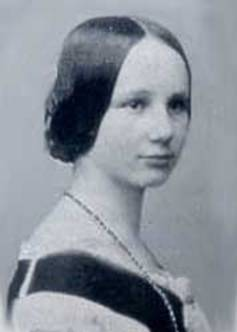
\includegraphics[scale=0.45]{./images/Lovelace}
    \end{column}
    \end{columns}

    \begin{block}{}
        Ada Lovelace est considérée par les informaticiens comme la première programmeuse de l'histoire.
    \end{block}
    
    \vfill
    
    C'est en son 
    honneur que le ministère américain de la Défense a appelé Ada un langage de programmation conçu par
    une équipe de Bull.
    
    \hfill \hyperlink{http://fr.wikipedia.org/wiki/Ada_Lovelace}{\beamergotobutton{Wikipedia}}

\end{frame}

% ------------------------- Sous-section --------------------------------------
\subsection{Les tubes à vide (1945 -- 1955)}

% ------------------------- Sommaire  --------------------------------------
\begin{frame}

	\frametitle{Plan}
	
	\tableofcontents[currentsubsection]
\end{frame}

% ------------------------- Diapo ----------------------------------------------
\begin{frame}
    \frametitle{Alan Turing (1912 -- 1954)}
    \begin{columns}
    \begin{column}{0.65\textwidth}
     \begin{itemize}
        \item Il est l'auteur, en 1936, d'un article de logique mathématique qui est devenu plus tard un 
        texte fondateur de la science informatique.
        \item Il a imaginé une machine théorique, la \og machine de Turing \fg, afin de donner une définition 
        précise au concept d’algorithme.
        \item Durant la Seconde Guerre mondiale, il a joué un rôle majeur dans les recherches sur les 
        cryptographies générées par la machine \alert{Enigma}, utilisée par les nazis.\\ Ces recherches
        conduirent à la construction du premier ordinateur électronique : \alert{COLOSSUS} (resté secret
        militaire pendant 30 ans) (1943).
        
        \hfill \hyperlink{http://fr.wikipedia.org/wiki/Alan_Turing}{\beamergotobutton{Wikipedia}}
     \end{itemize}
    \end{column}
    
    \begin{column}{0.35\textwidth}
        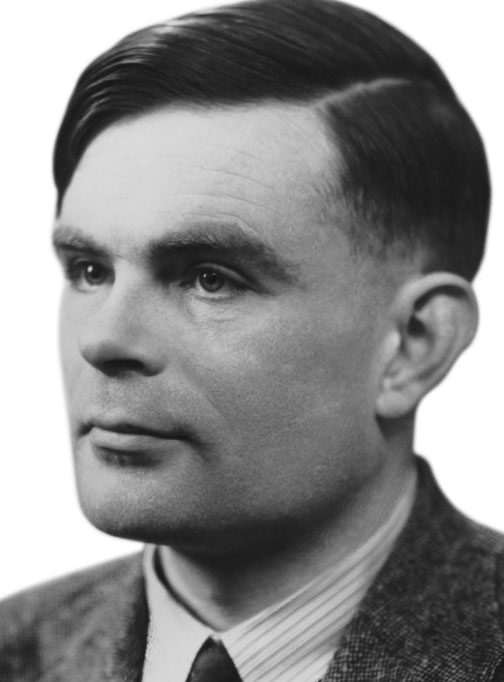
\includegraphics[scale=0.3]{./images/Turing}
    \end{column}
    \end{columns}
    
\end{frame}


% ------------------------- Diapo ----------------------------------------------
\begin{frame}
    \frametitle{ENIAC (Electronic Numerical Integrator Analyser and Computer) I}
    
    \begin{itemize}
        \item L'ENIAC fut le premier ordinateur entièrement électronique construit pour être Turing-complet
         (1946). 
        Il pouvait être reprogrammé pour résoudre, en principe, tous les problèmes calculatoires.
        
        \item L'ENIAC fut construit par John William Mauchly, professeur de physique, aidé par un de ses
        étudiants en thèse, J. Presper Eckert.
        
        \item L'ENIAC machine comportait 18\,000 tubes à vide et 1\,500 relais. Elle pesait 30 tonnes et 
        consommait 140~kW.
        
        \item L'ENIAC disposait de 20 registres de 10 \alert{chiffres décimaux} et on la programmait en manipulant
        quelques 6\,000 commutateurs interconnectés par une forêt de câbles. 
    \end{itemize}
    
    \hfill \hyperlink{http://fr.wikipedia.org/wiki/ENIAC}{\beamergotobutton{Wikipedia}}
\end{frame}


% ------------------------- Diapo ----------------------------------------------
\begin{frame}
    \frametitle{ENIAC (Electronic Numerical Integrator Analyser and Computer) II}   
    \begin{center}
        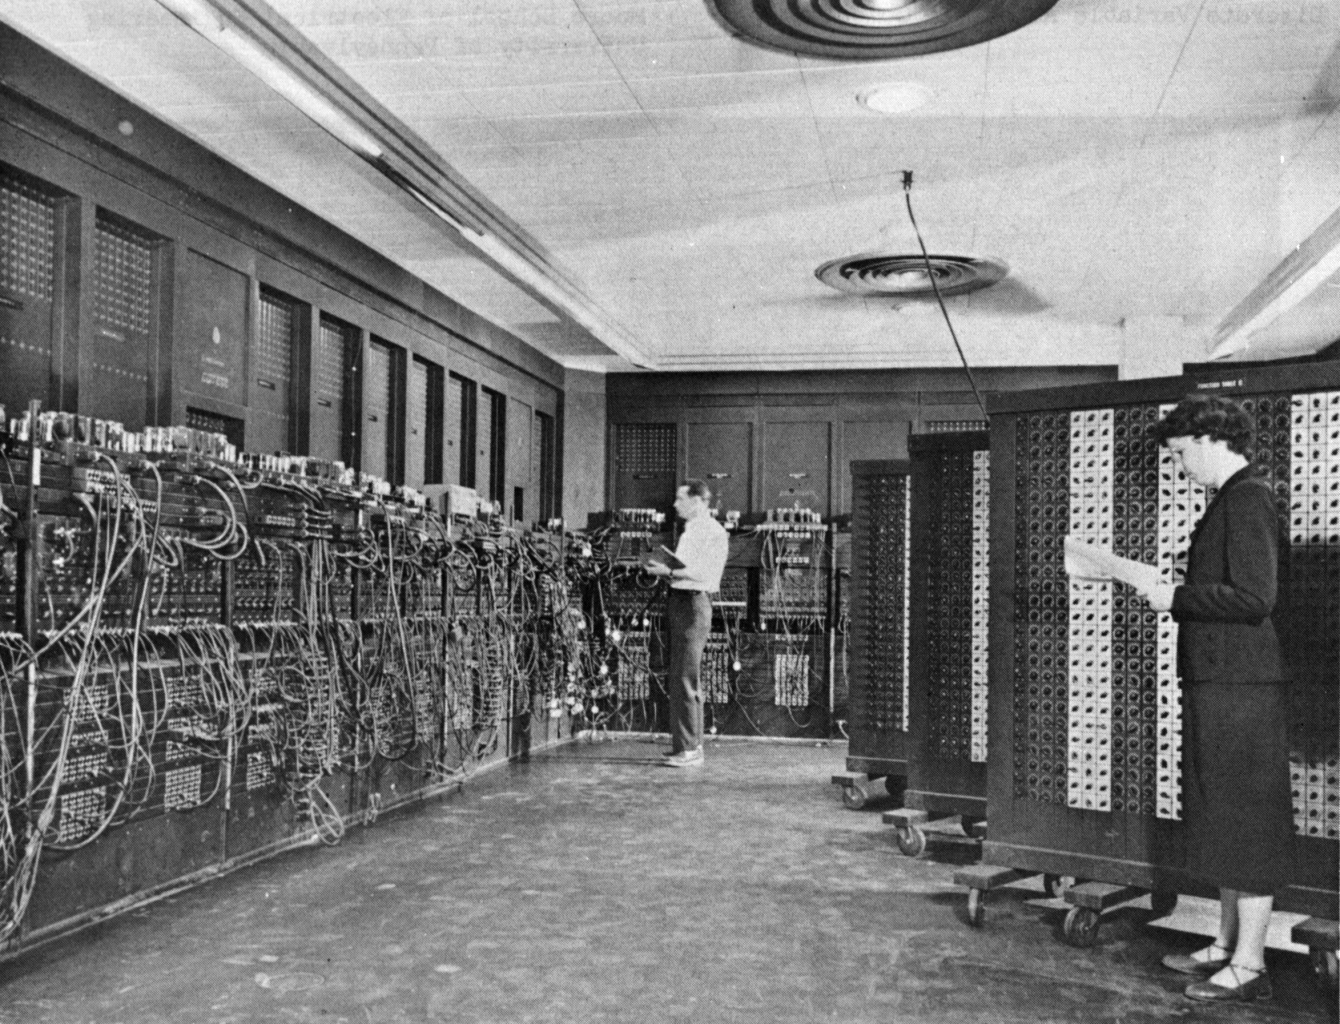
\includegraphics[scale=0.2]{./images/Eniac}
    \end{center}
\end{frame}

% ------------------------- Diapo ----------------------------------------------
\begin{frame}
    \frametitle{ENIAC (Electronic Numerical Integrator Analyser and Computer) III}
    \begin{center}
        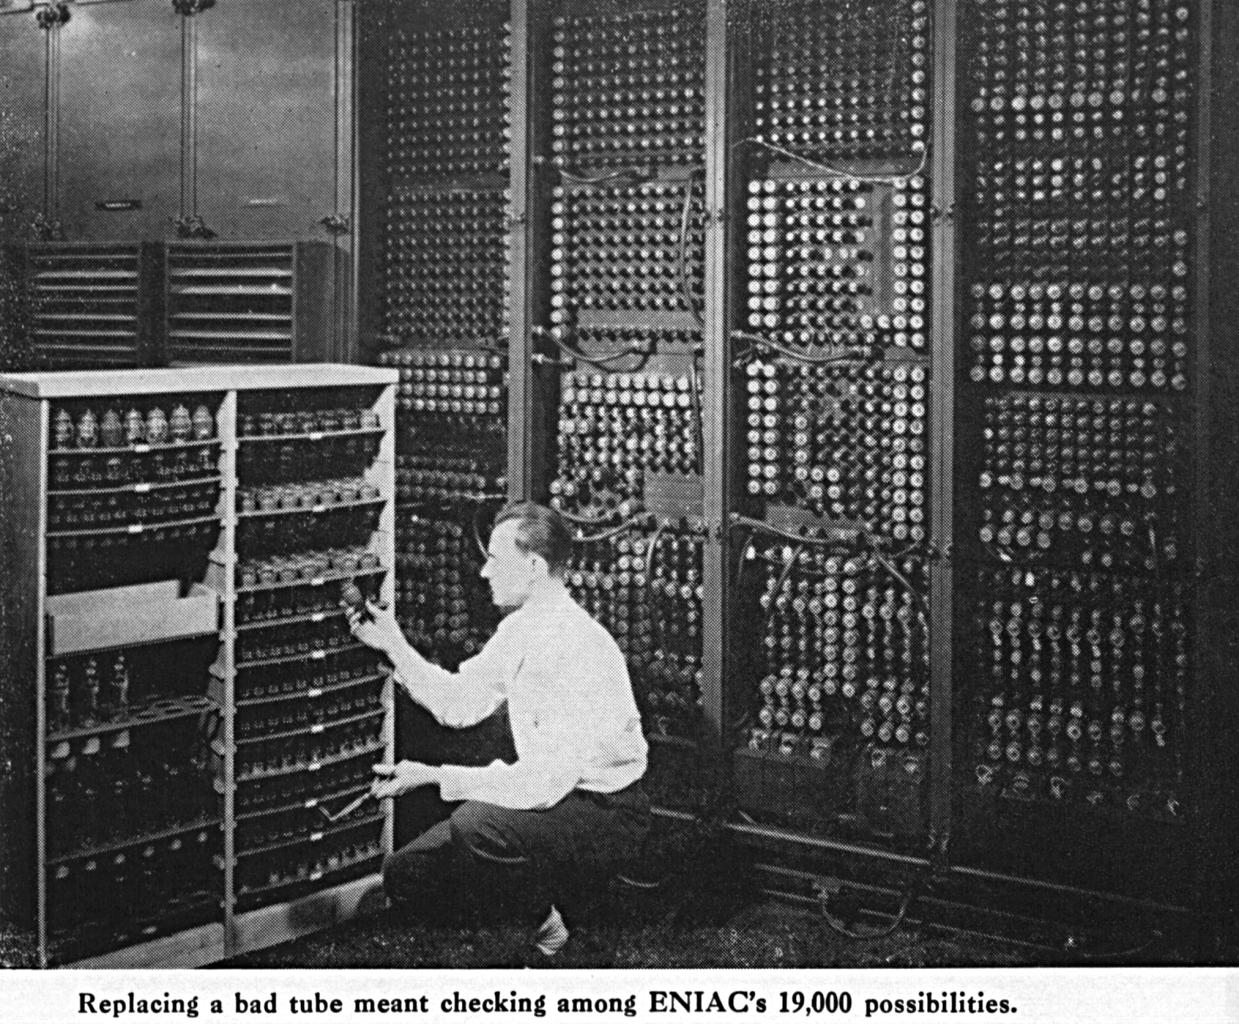
\includegraphics[scale=0.2]{./images/ENIAC-changing_a_tube}
    \end{center}
\end{frame}

    
% ------------------------- Diapo ----------------------------------------------
\begin{frame}
    \frametitle{ENIAC (Electronic Numerical Integrator Analyser and Computer) IV}    
    \begin{center}
    {\footnotesize
        \begin{tabular}{p{0.35\textwidth} p{0.3\textwidth} p{0.3\textwidth}}
        \toprule
        Moyen employé&	Vitesse de multiplication de nombres de 10 chiffres	& Calcul d'une trajectoire 
        d'une table de tir \\
        \toprule
        Homme à la main, ou machine de Babbage & \el{5 min} & \el{2,6 jours} \\
        \midrule
        Homme avec calculateur de bureau & \el{10 à 15 secondes} & \el{12 heures} \\
        \midrule
        Harvard Mark I (électromécanique) & \el{3 secondes} & \el{2 heures} \\
       \midrule
        Model 5 (électromécanique) & \el{2 secondes} & \el{40 minutes}  \\
        \midrule
        Analyseur différentiel (analogique) & \el{1 seconde} & \el{20 minutes} \\
        \midrule
        Harvard Mark II (électromécanique) & \el{0,4 s} & \el{15 minutes} \\
        \midrule
        ENIAC (électronique)	 & \el{0,001 s} & \el{3 secondes}\\
        \bottomrule
        \end{tabular}
    }
    \end{center}


\end{frame}

% ------------------------- Diapo ----------------------------------------------
\begin{frame}
    \frametitle{John von Neumann (1903 -- 1957)} 
    
    \begin{columns}
    \begin{column}{0.6\textwidth}
     \begin{itemize}
        \item Il comprit que la programmation des ordinateurs dotés d'un très grand nombre de commutateurs
         était trop
        lente, fastidieuse et rigide.
        \item Il proposa de représenter le programme sous forme numérique et de le stocker dans la
        mémoire, au même titre que les données.
        \item Il proposa de remplacer l'\alert{arithmétique décimale} série de l'ENIAC, dans laquelle chaque chiffre 
        est représenté par dix tubes à vide (1 allumé et 9 éteints) par une \alert{arithmétique binaire parallèle}.        
     \end{itemize}
    \end{column}
    \begin{column}{0.4\textwidth}
            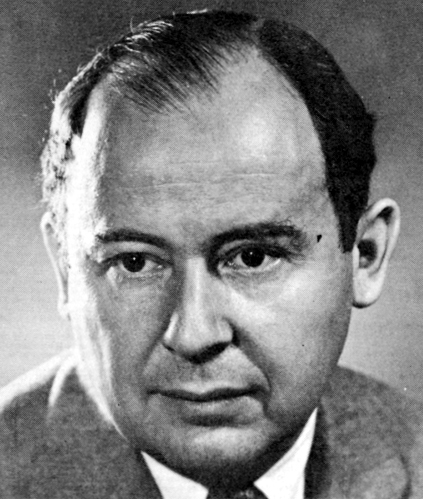
\includegraphics[scale=0.28]{./images/JohnvonNeumann-LosAlamos}
    \end{column}
    \end{columns}
    \begin{block}{}
        Von Neumann a donné son nom à l'\alert{architecture de von Neumann} utilisée dans la quasi-totalité des ordinateurs modernes.
    \end{block}
    
    \hfill \hyperlink{http://fr.wikipedia.org/wiki/Alan_Turing}{\beamergotobutton{Wikipedia}}

\end{frame}

% ------------------------- Diapo ----------------------------------------------
\begin{frame}
    \frametitle{Machine de von Neumann}
    \framesubtitle{EDSAC : premier ordinateur à programme enregistré}
     
     \begin{columns}
    \begin{column}{0.5\textwidth}
        \begin{description}
            \item [Mémoire :] 4096 mots de 40 bits, donc deux instructions de 20 bits ou un entier signé de
            39 bits.
            \item 
        \end{description}

    \end{column}
    
    \begin{column}{0.5\textwidth}
        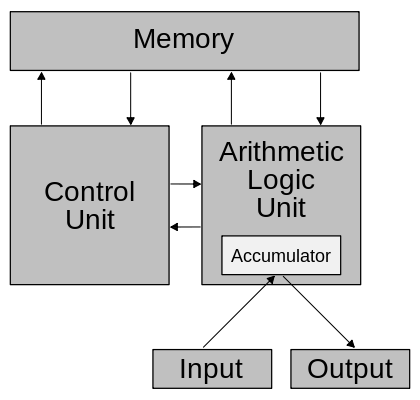
\includegraphics[scale=0.4]{./images/Von_Neumann_architecture}
    \end{column}
    \end{columns}
    
\end{frame}

% ------------------------- Diapo ---------------------------------------------
\begin{frame}
	\frametitle{Grace Hopper (1906 -- 1992)}
	
	\hfill 
	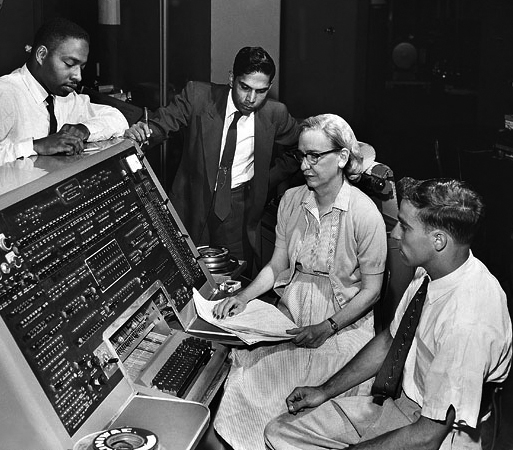
\includegraphics{images/Grace_Hopper_and_UNIVAC}
	\hfill
	\includegraphics[scale=0.15]{images/Commodore_Grace_M_Hopper}
	\hfill \\
	
	\begin{block}{}
        À partir de 1957, Grace Hopper défend l'idée qu'un programme devrait pouvoir être écrit dans un langage proche de l'anglais plutôt que d'être calqué sur le langage machine, comme l'assembleur. De cette idée naît le langage COBOL en 1959.
    \end{block}
    
    \begin{flushright}
        \hyperlink{http://fr.wikipedia.org/wiki/Grace_Hopper}%
            {\beamergotobutton{Wikipedia}}
    \end{flushright}

\end{frame}

% ------------------------- Diapo ---------------------------------------------
\begin{frame}
    \frametitle{Bug informatique}
    
    \begin{columns}
    \begin{column}{0.5\textwidth}
        Expression popularisée suite à la panne d'un ordinateur Mark II due à un papillon de nuit, de l'anglais moth, pris dans un relais. L’insecte, \og bug \fg\ en anglais, fut enlevé avec soin et placé dans le journal de bord avec la mention \og \alert{first actual case of bug being found} \fg\ (premier cas réel de découverte d'insecte). 
    \end{column}
    
    \begin{column}{0.5\textwidth}
        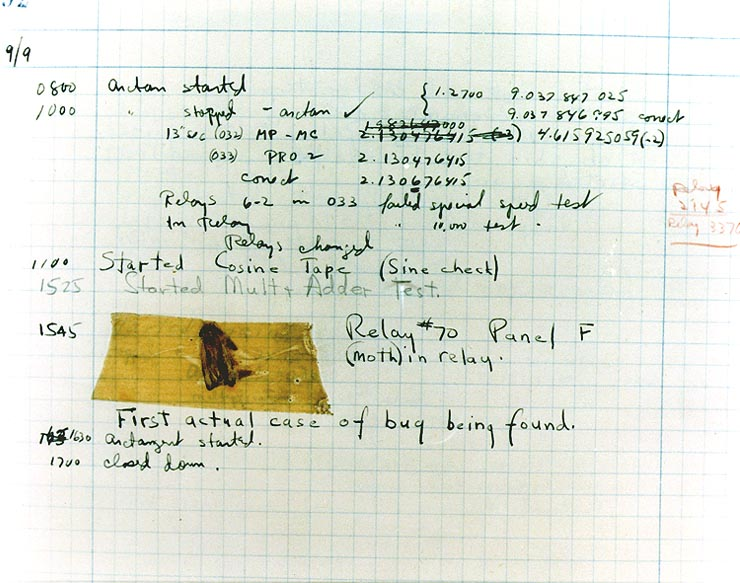
\includegraphics[scale=0.3]{./images/Bug}
    \end{column}
    \end{columns}
\end{frame}

% ------------------------- Sous-section --------------------------------------
\subsection{Les transistors (1955 -- 1965)}

% ------------------------- Sommaire deuxième section --------------------------------------
\begin{frame}

	\frametitle{Plan}
	
	\tableofcontents[currentsubsection]
\end{frame}


% ------------------------- Sous-section --------------------------------------
\subsection{Les circuits intégrés (1965 -- 1980)}

% ------------------------- Sommaire deuxième section --------------------------------------
\begin{frame}

	\frametitle{Plan}
	
	\tableofcontents[currentsubsection]
\end{frame}


% ------------------------- Sous-section --------------------------------------
\subsection{Les ordinateurs personnels (1980 -- ?)}

% ------------------------- Sommaire deuxième section --------------------------------------
\begin{frame}

	\frametitle{Plan}
	
	\tableofcontents[currentsubsection]
\end{frame}

% ------------------------- Section --------------------------------------
\section{Structure d'un ordinateur}


% ------------------------- Sous-section --------------------------------------
\subsection{L'Unité Centrale}

% ------------------------- Sous-section --------------------------------------
\subsection{La mémoire}

% ------------------------- Sous-section --------------------------------------
\subsection{Les périphériques}

% ------------------------- Fin du document ----------------------------------------
\end{document}